\documentclass[10pt,a4paper]{article}
\usepackage[margin=1.8cm]{geometry}
\usepackage{amsmath,amssymb}
\usepackage{booktabs}
\usepackage{tabularx}
\newcolumntype{L}{>{\raggedright\arraybackslash}X}
\usepackage{graphicx}
\usepackage{float}
\usepackage[T1]{fontenc}
\usepackage{microtype}
\usepackage[colorlinks,linkcolor=black,citecolor=black,urlcolor=blue]{hyperref}
\usepackage[dvipsnames]{xcolor}
\usepackage{titlesec}
\definecolor{passgreen}{rgb}{0.05,0.50,0.20}
\definecolor{failred}{rgb}{0.72,0.13,0.13}
\newcommand{\PASS}[1]{\textcolor{passgreen}{\textbf{#1}}}
\newcommand{\FAIL}[1]{\textcolor{failred}{\textbf{#1}}}
\newcommand{\PEND}[1]{\textcolor{gray}{#1}}
\titlespacing*{\section}{0pt}{6pt}{2pt}
\newcommand{\code}[1]{\texttt{#1}}
\newcommand{\op}[1]{\texttt{#1}}
\title{\vspace{-1.4cm}\textbf{The basement membrane as a surface with a reservoir:\\
\normalsize deformation, remeshing, tearing, and the Plexus2 container they live in}}
\author{}
\date{\vspace{-0.9cm}\small \texttt{prototype/ecm/bm\_ops.py} $\cdot$
\texttt{test\_05\_sheet.py} $\cdot$ \texttt{test\_05b\_plaque.py} $\cdot$
\texttt{test\_05c\_remesh.py} $\cdot$ \texttt{test\_05e\_conserve.py} $\cdot$
\texttt{log/okuda\_ECM/05a--05c} \ (\texttt{05d--05f} archived, see \S4.2) $\cdot$ 10 August 2026}
\setlength{\parindent}{0pt}\setlength{\parskip}{0.55em}
\begin{document}\maketitle\vspace{-1.0cm}

\section*{1.\; Mechanism}

\textbf{What the object is.} A basement membrane is a sheet of crosslinked protein --- collagen~IV
and laminin, with nidogen and perlecan --- about $100$ nm thick, that an epithelium secretes onto its
own basal surface and then sits on. Every epithelium in the body has one. It is the boundary that
makes a tissue a tissue: it separates epithelium from stroma, carries the mechanical load of the sheet
above it, holds growth factors, passes solutes while stopping cells, and is the thing a tumour must
breach to become invasive.

\textbf{What it has to do, and why the two demands conflict.} It must \emph{hold together as a
material}, which asks it to be stiff and continuous; and it must \emph{keep covering a surface that
grows}, which for the spheroid modelled here means an area rising by a factor of eleven. Those pull
against each other, and biology resolves them with three mechanisms rather than with a compromise in
stiffness:

\begin{itemize}\itemsep1pt
\item \textbf{it is replaced while it is stretched.} Collagen~IV turns over on a half-life of
      $3$--$10$ hours \cite{matsubayashi2020}, comparable to the time in which the tissue grows, so the
      sheet enclosing a tripled radius is not the sheet that was there at the start.
\item \textbf{it is attached, not merely adjacent.} Integrin clusters bind it to the cells beneath,
      transmitting traction both ways and letting the sheet slide as the tissue rearranges underneath.
\item \textbf{it fails where it is not resupplied.} A hole is not a stress concentration on a fixed
      material; it is a place where removal beat deposition.
\end{itemize}

\textbf{The equations those mechanisms are, before any discretisation.} Each is a balance on a
quantity carried per unit area of a deforming surface, and each has the same shape --- a material
derivative, a source, a sink, and a dilution term that appears because the surface itself is growing:

\begin{center}\small
\begin{tabular}{@{}lll@{}}\toprule
carried quantity & balance & what it decides\\\midrule
sheet material $\rho$ & $\mathrm D\rho/\mathrm Dt = s-\rho/\tau_{\rm bm}-\rho\,\dot A/A$ &
  whether the sheet thins, holds, or tears\\
receptor $n_f$, bonds $n_b$ & binding kinetics with a load-dependent off-rate &
  how hard it is held, and whether it slides\\
momentum & $\gamma\dot{\mathbf x}=\mathbf f$, massless and overdamped &
  where it sits and how fast it gets there\\
\bottomrule
\end{tabular}
\end{center}

\textbf{Why the mechanics is overdamped and not inertial.} At the scale of a membrane in tissue fluid
the Reynolds number is $\sim\!10^{-10}$: inertia is not small, it is absent. The correct statement of
motion is that velocity is proportional to force, and the consequence for everything downstream is
that a \emph{stiffness has no meaning on its own} --- only the ratio $k/\gamma$, a relaxation rate,
appears. The question a stiffness answers here is not ``how strong'' but ``does the sheet relax faster
than the tissue grows''.

\textbf{What this becomes in Plexus2.} A model is sets $\times$ fields $\times$ operators $\times$
schedule, and the biology above chooses all four. The sheet is a \emph{surface}, so it is a node set
(\code{bm}) with a hyperedge set of triangles over it (\code{bm\_face}) that carries everything
material; its thickness never becomes geometry, only a coefficient. Adhesion is a \emph{relation
between two entities}, so it is an edge set (\code{plaque}) whose single operator returns a force to
both ends and cannot get them out of step. The receptor belongs to the \emph{cell}, so it is a state
on \code{cell}. And because the sheet gains and loses material, its \emph{size is a state variable}:
the sets are allocated with a reserve and carry the framework's \code{occ} flag, exactly as MPM
particles do for \op{cell\_grow}.

\textbf{One distinction is load-bearing throughout this note.} \op{bm\_refine} --- changing the
triangulation as the surface grows --- is a \emph{numerical} operation. It changes no physical
quantity: not the surface, not the material state, not the mass. Secretion, turnover and proteolysis
are \emph{biological} mechanisms that change what the sheet is made of and how much there is. They
share an implementation substrate, the \code{occ} reservoir, and nothing else. Conflating them is what
lets a discretisation choice be read as a result --- and the historical case is exactly that: the
previous implementation of this sheet, as material points on a background grid, produced tearing that
was set by the grid spacing rather than by any stress, on a sheet an eighth of a grid cell thick. \S4
gives the gate that catches it and the measurement that passes it.

\textbf{How the rest reads.} \S2 gives the equations from the coarsest statement down: the balance of
forces on the surface, then the elasticity and the strain measure it needs, then the material budget,
then the adhesion, then the discretisation. \S3 writes all of it as a Plexus2 container --- sets,
states, operators, schedule. \S4 is the gate table: every claim in \S2 with a threshold fixed before
the run and the number that came back.

\section*{2.\; Equations and symbols}

\textbf{The whole model, in one line, before any of it is expanded.} The sheet is a massless
overdamped surface, so its equation of motion is a balance between the forces acting on it and the drag
resisting them:
%
\begin{equation}
\gamma\,\dot{\mathbf x} \;=\;
\underbrace{\mathbf f_{\rm el}}_{\text{\S2.1: it is elastic}}
\;+\;\underbrace{\mathbf f_{\rm adh}}_{\text{\S2.3: it is attached}}
\;+\;\underbrace{\mathbf f_{\rm con}}_{\text{\S2.3: it is outside the cells}},
\qquad
\mathbf x\leftarrow\mathbf x+\Delta t\,M\,\mathbf f,\quad M=1/\gamma,
\label{eq:motion}
\end{equation}
%
alongside two budgets on quantities the surface carries --- its own material (\S2.2) and the bonds
holding it (\S2.3) --- and one statement about the mesh that carries none of it (\S2.4).

\textbf{The stability limit that follows, because it constrains every term above.} With no mass there
is no wave speed, so the limit is a \emph{rate}:
%
\begin{equation}
\boxed{\ \Delta t\,M\,\lambda_{\max}(\mathbf H)<2\ },
\label{eq:step}
\end{equation}
%
$\mathbf H$ being the Hessian of the energy. This is about twenty times weaker than the CFL an inertial
sheet would carry, which is why a membrane ten to a hundred times stiffer than the stroma does not set
the timestep for the whole model. $\lambda_{\max}$ is \emph{measured}, by power iteration on
Hessian-vector products, and re-measured as the run proceeds: a St~Venant--Kirchhoff membrane's tangent
stiffens as it stretches, and over $401$ frames it grew $19.1\times$ ($4.56\to87.2$), taking the substep
count with it ($21\to194$). Fixing the substep count from the seeded value put the measured divergence
threshold at $1.8$ instead of $2$, and the entire discrepancy was the Hessian having grown under the
run's own load.

\subsection*{2.1\; The elastic surface, and the strain measure it needs}

The first term of Eq.~\eqref{eq:motion} is the sheet resisting being stretched. One constant-strain
triangle per face, St~Venant--Kirchhoff, thickness entering only as a multiplier:
%
\begin{align}
W_f &= A^0_f\Bigl[\mu\operatorname{tr}\bigl(\mathbf E_g^2\bigr)
      +\tfrac{\Lambda}{2}\bigl(\operatorname{tr}\mathbf E_g\bigr)^2\Bigr],
&\mathbf E_g&=\tfrac12\bigl(\mathbf C_{\rm el}-\mathbf I\bigr),
&\mathbf f&=-\frac{\partial}{\partial\mathbf x}\sum_f W_f ,
\label{eq:energy}\\[2pt]
Y_2&=E\,T\quad\text{[force per unit \emph{length}]},
&\mu&=\frac{Y_2}{2(1+\nu)},
&\Lambda&=\frac{Y_2\,\nu}{1-\nu^2} .
\label{eq:moduli}
\end{align}
%
The force is the exact gradient, taken by automatic differentiation, so the force and the energy cannot
disagree --- G4 checks it against a central finite difference and gets $5\times10^{-10}$ relative.

\textbf{Which needs a strain measure, and this is the one the whole note is written in.}
$\lambda$ is the quantity every other statement here is written in, and it is a \emph{per-triangle}
number. For a face with nodes $\mathbf x_{0,1,2}$, take the two edge vectors from the first node now and
in the reference configuration $\mathbf X$:
%
\begin{equation}
\mathbf D_s = \bigl[\,\mathbf x_1-\mathbf x_0,\;\mathbf x_2-\mathbf x_0\,\bigr]\in\mathbb R^{3\times2},
\qquad
\mathbf D_m = \begin{bmatrix} a & \mathbf v\!\cdot\!\hat{\mathbf e}_1\\[2pt]
0 & \mathbf v\!\cdot\!\hat{\mathbf e}_2\end{bmatrix}\in\mathbb R^{2\times2},
\label{eq:frames}
\end{equation}
%
where $\mathbf D_m$ is the same pair written in the reference triangle's \emph{own} in-plane frame
$(\hat{\mathbf e}_1,\hat{\mathbf e}_2)$, with $a=|\mathbf X_1-\mathbf X_0|$ and $\mathbf v=\mathbf X_2-
\mathbf X_0$. Then
%
\begin{equation}
\mathbf F = \mathbf D_s\mathbf D_m^{-1}\in\mathbb R^{3\times2},\qquad
\mathbf C = \mathbf F^{\!\top}\mathbf F,\qquad
\lambda_{1,2}=\sqrt{\operatorname{eig}\mathbf C},\qquad
J=\lambda_1\lambda_2=\frac{\text{area now}}{\text{area then}} .
\label{eq:lambda}
\end{equation}
%
$\lambda_1$ is the larger principal stretch: $1$ is unstretched. \textbf{This is what the movies colour
by} --- \code{lam} in \code{traj.npz}, \code{lam\_geo} in \code{metrics.json}. Because $\mathbf F$ is
read from where the nodes \emph{are} against where they \emph{were}, it is blind to what moved them: a
node moved by a tether, a plaque, a grid or by hand is seen identically, and there is no path by which a
displacement is applied and not counted. That is a property of Eq.~\eqref{eq:lambda} and not a result,
which is why it can be certified in closed form (\S4, G1--G4) before any physics runs.

\textbf{There are two $\lambda$'s and they must never be quoted as one.} The reference metric is either
frozen at seeding or allowed to creep (\S4), giving
%
\begin{equation}
\lambda^{\rm geo}=\sqrt{\operatorname{eig}\mathbf C}\ \ \text{(against the SEEDED metric)},
\qquad
\lambda^{\rm el}=\sqrt{\operatorname{eig}\bigl(\mathbf C_0^{-1}\mathbf C\bigr)}\ \
\text{(against the REMEMBERED metric $\mathbf C_0$)} .
\label{eq:twolambda}
\end{equation}
%
$\lambda^{\rm geo}$ is what the tissue did to the sheet; $\lambda^{\rm el}$ is what the material feels.
With no remodelling they coincide. With remodelling they do not, and the gap is the mechanism.

\subsection*{2.2\; Memory, stiffening, supply}


\textbf{Remodelling} is the reference metric creeping toward the current one, the 2D form of the
archived per-edge $\dot\ell^0=(L-\ell^0)/\tau_r$:
%
\begin{equation}
\mathbf C_0\leftarrow\mathbf C_0+\frac{\Delta t}{\tau_r}\bigl(\mathbf C-\mathbf C_0\bigr).
\label{eq:remodel}
\end{equation}
%
Collagen~IV's half-life of $3$--$10$ hours is $13$--$93$ frames here, so this is resolved rather than
instantaneous. A sheet enclosing a surface that triples in radius cannot do it elastically.

\textbf{Strain stiffening}, $E(\lambda)=E_0[1+\beta(\lambda^{\rm el}-1)]$, applied explicitly from the
previous step's stretch so that Eq.~\eqref{eq:energy} remains the exact potential of the force.
Candiello \emph{et al.} measure $0.4\to3$~MPa on native basement membrane; \textbf{MPa is not a quantity
this box has} --- it is dimensionless and the stroma's modulus is the number $15$ --- so the falsifiable
forms are the ratio $E(\lambda_{\max})/E_0$ and the contrast $E_{\rm bm}/E_{\rm ecm}\in[10,100]$.

\textbf{Areal density, and which of the two is the state.} The mass balance a growing sheet owes is
usually written for $\rho$,
%
\begin{equation}
\frac{\mathrm D\rho}{\mathrm Dt}=\underbrace{s(\mathbf x,t)}_{\text{secretion}}
-\underbrace{\frac{\rho}{\tau_{\rm bm}}}_{\text{turnover}}
-\underbrace{\rho\frac{\dot A}{A}}_{\text{dilution}},\qquad
s^\ast=\rho\Bigl(\frac1{\tau_{\rm bm}}+\frac{\dot A}{A}\Bigr),
\label{eq:mass}
\end{equation}
%
whose two removal terms are the same size here ($\sim\!10^{-1}\,$h$^{-1}$ each) --- turnover is not a
correction to growth, it is the same size as growth, which is why a sheet can accommodate growth at all.

\textbf{But $\rho$ is the wrong variable to store, and 05e is the run that changed it.} Carry the
\emph{mass} $m_f$ on each face and derive the density,
%
\begin{equation}
\rho_f=\frac{m_f}{A_f(\text{now})},\qquad
\frac{\mathrm d m_f}{\mathrm dt}=s\,A_f-\frac{m_f}{\tau_{\rm bm}},
\label{eq:massstate}
\end{equation}
%
and three things follow that the $\rho$ form does not give. The dilution term \emph{disappears from the
integration} --- it is what dividing by a growing area does on its own, and Eq.~\eqref{eq:mass}
integrated alongside Eq.~\eqref{eq:massstate} would count it twice. $\sum_f m_f$ becomes a conserved
quantity that only secretion and proteolysis may change, so a remesh can be \emph{gated} on it (G18b,
measured bit-identical). And run 128's failure mode becomes structurally impossible: mass is added to
faces that already are the sheet, so there is no way to secrete material into the lumen.

With $s=0$ the measured sheet thins to $1/11.1$ of what it was seeded with, which is
Eq.~\eqref{eq:massstate} with no source and an area $\times11.1$. \textbf{That number is the baseline
\op{bm\_secrete} has to hold flat}, and it is the reason a fixed particle budget was never going to
work.

\subsection*{2.3\; Adhesion: a receptor on the cell, bonds on the edge, ligand on the sheet}

\begin{figure}[H]\centering
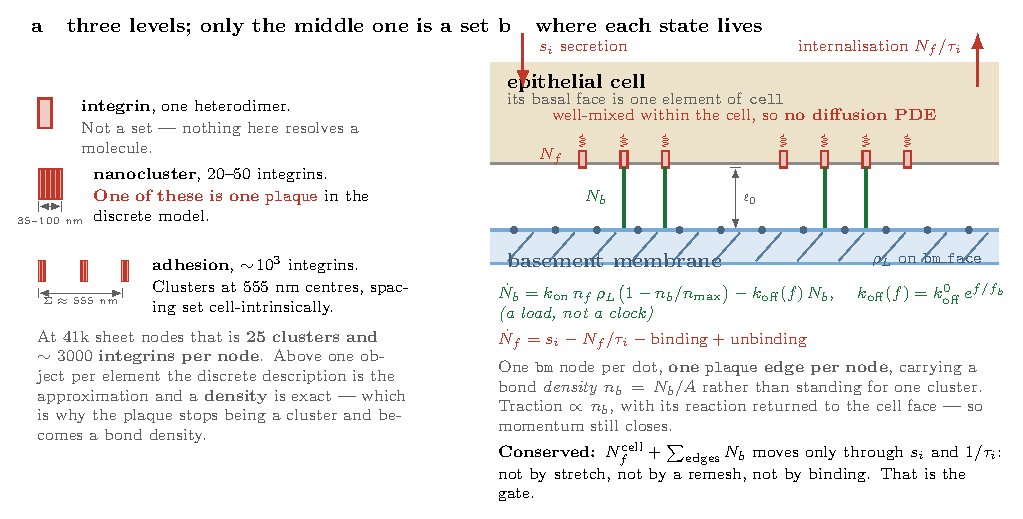
\includegraphics[width=\textwidth]{fig_adhesion_scheme.pdf}
\caption{\textbf{(a)} An integrin is a heterodimer; $20$--$50$ of them make a nanocluster
$35$--$100$ nm across \cite{changede2017}; clusters group into adhesions of $\sim\!10^3$ integrins at a
measured $\sim\!555$ nm centre-to-centre spacing \cite{nanoclusters2025}. The discrete \op{plaque} of
05b was the MIDDLE level --- one cluster --- and at $41$k sheet nodes there are $25$ clusters and
$\sim\!3000$ integrins per node, so that description was resolving something the mesh cannot see.
\textbf{(b)} The three states, each on the entity it belongs to. Free receptor is the CELL's and is
well mixed over its own basal face; bonds are a relation and live on the edge; ligand is sheet
material and is already $\rho$.}
\end{figure}

\textbf{A plaque is not an integrin; it is a cluster of them, and that hierarchy decides where every
state goes.} An integrin is a single transmembrane heterodimer. Integrins do not act alone --- they
assemble into \emph{nanoclusters} of $20$--$50$ molecules, $35$--$100$ nm across, which is what lets an
adhesion carry load no single bond could \cite{changede2017} --- and those clusters group into an
adhesion of order $10^3$ integrins, spaced $\sim\!555$ nm centre to centre by a cell-intrinsic
mechanism rather than by the ligand \cite{nanoclusters2025}.

\textbf{The arithmetic then decides the representation, and it decides against discrete plaques.} This
sheet is $0.317$ mm$^2$ at the last frame. At the measured spacing that is $\sim\!1.03\times10^6$
clusters --- against $40{,}962$ nodes. \textbf{Twenty-five clusters and $\sim\!3000$ integrins per
node}, with a shot noise of $2\%$: above one object per element the discrete description is the
approximation and the density is exact. 05b's $1166$ plaques were not a sparse sampling of adhesion,
they were the wrong object by a factor of $883$.

\textbf{So the receptor becomes a field, and it belongs to the cell.} An integrin is a protein in the
\emph{cell's} basal plasma membrane; the sheet carries the \emph{ligand}. Three states, each on the
entity that owns it:

\smallskip
{\footnotesize
\begin{tabularx}{\textwidth}{@{}llL@{}}\toprule
state & lives on & dynamics\\\midrule
$N_f$, free receptor & \code{cell}, its basal face & $\dot N_f=s_i-N_f/\tau_i-\text{binding}
  +\text{unbinding}$ --- production and internalisation, no flux term (below)\\
$N_b$, bound bonds & \textbf{edge} \code{plaque}: \code{cell}$\to$\code{bm} & Eq.~\eqref{eq:clutch}:
  a bond has two ends, so it is a relation and not a state of either body\\
$\rho_L$, ligand & \code{bm\_face} & laminin is sheet material; this is $\rho$, already there\\
\bottomrule
\end{tabularx}}
\smallskip

\textbf{And putting the receptor on the cell removes the PDE rather than adding one.} The plasma
membrane is continuous within a cell and interrupted at cell--cell junctions, so integrins do not
diffuse between cells --- lateral transport between them is exocytosis and endocytosis, a per-cell
source and sink, not a flux. \emph{Within} one cell, at $D\approx0.1\,\mu$m$^2$/s over a $600$ s frame,
a receptor explores $\sqrt{4Dt}=15.5\,\mu$m against a $\sim\!10\,\mu$m cell: the basal face is
\textbf{well mixed at our timestep}. So there is no Laplacian, no $\Delta t D/h^2<\tfrac12$ constraint
--- which would have cost $\sim\!14$ substeps and, unlike the sheet's rate bound, would have
\emph{tightened} at every refinement --- and the receptor obeys a per-cell ODE. The assumption is
stated rather than silent: if a cell is ever resolved by more than one face, the diffusion term returns.

The bonds themselves are the classical clutch, with Bell's force-dependent unbinding:
%
\begin{equation}
\dot N_b = k_{\rm on}\,n_f\,\rho_L\Bigl(1-\frac{n_b}{n_{\max}}\Bigr)A
 \;-\; k_{\rm off}(f)\,N_b,
\qquad k_{\rm off}(f)=k^0_{\rm off}\,e^{f/f_b},
\qquad n_b=\frac{N_b}{A},
\label{eq:clutch}
\end{equation}
%
and the traction on the sheet is $\propto n_b$, with the reaction returned barycentrically to the
cell's face exactly as \op{plaque\_pull} does now --- so G9 and G10 keep passing unchanged. \textbf{The
\op{plaque} edge set survives and is reinterpreted}: one edge per sheet node, taken from the
\op{bm\_contact} map, carrying a bond \emph{density} for its patch rather than standing for one
cluster.


\textbf{The force those bonds exert, and one sign that cost a run.} The normal law is a spring at the
linkage's own rest length, scaled by how many bonds the patch is carrying, and the tangential law is
friction against the relative velocity of sheet and cell:
%
\begin{align}
\mathbf f_n &= -\,n_b\,\kappa_n\,(d-\ell_0)\,\hat{\mathbf n},
&d &= (\mathbf x^{\rm bm}-\mathbf p)\cdot\hat{\mathbf n},
&\mathbf f^{\rm epi}_k &= -w_k(\mathbf f_n+\mathbf f_t),
\label{eq:plaque_n}\\[2pt]
\dot{\mathbf x}_\parallel &=
\frac{\dot{\mathbf x}^{\rm prov}_\parallel+M\xi\,\mathbf v^{\rm epi}_\parallel}{1+M\xi},
&\xi &= n_b\kappa_b/k_{\rm off},
&\mathbf f_t &= \xi\bigl(\mathbf v^{\rm epi}_\parallel-\dot{\mathbf x}_\parallel\bigr).
\label{eq:implicit}
\end{align}
%
$\hat{\mathbf n}$ is the epithelial face's \emph{outward} normal, not the line joining the two points,
and that is a correctness fix rather than a refinement: along the line, the equilibrium
$|\mathbf x^{\rm bm}-\mathbf p|=\ell_0$ is satisfied on \emph{either} side, so a sheet that has sunk
through the epithelium sits at the same energy as one resting on it. 05e measured the consequence --- a
sheet that started $5.96\times10^{-4}$ outside (which is $\ell_0$, correct) and ended
$7.7\times10^{-3}$ \emph{inside}, thirteen $\ell_0$ through the cell layer --- while the standoff
metric, being an unsigned distance, reported $+4.0\times10^{-3}$ throughout. \textbf{An unsigned
quantity cannot answer a question about a side.}

Eq.~\eqref{eq:implicit} is \emph{solved}, not evaluated: an explicit $-\xi\mathbf v$ is a stiffness of
$\xi/\Delta t$, which \emph{grows} as the substep shrinks, so refining the step to stabilise it makes
it worse. And a signed adhesion is still not sufficient --- with the sign fixed the sheet ended
$89.6\%$ inside, because the missing statement is one no adhesion model contains:

\begin{equation}
\mathbf f^{\rm contact}_i=-k_c\,\min\bigl(d_i-\ell_0,\,0\bigr)\,\hat{\mathbf n}_i,
\qquad\text{one-sided, at every node.}
\label{eq:contact}
\end{equation}

\op{bm\_contact} says that a basement membrane cannot be \emph{inside} the cells. It holds at every
node and not only where adhesion happens to be, it pushes out and never pulls in, and its reaction goes
to the three vertices of the epithelial face so the momentum gate still covers it. It moved the signed
standoff from $-9.87\times10^{-4}$ to $+1.97\times10^{-6}$ and the fraction of nodes on the wrong side
from $89.6\%$ to $\mathbf{0.0\%}$. This is what the archived \op{cell\_exclude\_3d} did and got wrong:
that operator \emph{projected} particles out, repositioning them without touching $\mathbf F$, which
launders deformation --- run 88's sheet was carried outward as a decal at a strain of
$7\times10^{-4}$ against a true stretch of $3.4$. A force cannot do that.

\textbf{Three defects close at once, which is why this is a change of scheme and not an elaboration.}
The standoff (G12) was $3.43\,\ell_0$ because $96\%$ of nodes were unanchored and the sheet sagged
between plaques; a distributed traction has nothing to sag between. Slip (G13) was unmeasurable because
a fixed barycentric anchor is a tangential pin --- slip \emph{is} bond turnover, the sheet advancing as
$k_{\rm off}$ releases bonds that rebind ahead, and $\xi$ stops being a coefficient and becomes
$n_b\kappa_b/k_{\rm off}$. And rupture was a clock because a fixed threshold on a monotonically rising
load is reached by everyone eventually; $k_{\rm off}(f)$ gives a \emph{steady-state} bound fraction
that depends on load, so ``fraction bound versus stress'' becomes a curve.

\textbf{What is conserved, and therefore what is gated:} $N_f^{\rm cell}+\sum_{\rm edges}N_b$ changes
only through $s_i$ and $1/\tau_i$ --- not by stretch, not by a remesh, not by binding, which merely
moves receptor from one column to the other. That is the G18b treatment applied to receptor instead of
mass.

\textbf{The discrete plaque is not deleted; it is demoted to a refined patch.} Where individual rupture
and turnover matter --- a crack tip, an invadopodium --- a locally refined mesh can resolve $\Sigma$
and carry discrete clusters again. The gate on that is a convergence test: the discrete model at high
density must reproduce the density model.

\subsection*{2.4\; The reservoir: a sheet whose size is a state variable}


This is the part the archived line had no equivalent of, and it is what makes the rest possible.

\textbf{What a remesh is, and what it must never be.} \op{bm\_refine} is a numerical topology update.
The physical surface is unchanged --- the same points of space, the same enclosed volume, the same
material --- and so is everything the material knows about itself. It exists because a fixed
triangulation stops resolving a surface whose area grows by an order of magnitude, and for no other
reason. \textbf{Nothing biological may be inferred from a refinement, and no biological operator may be
implemented as one.} A tear that appears because the mesh was coarse, a thinning that appears because
triangles grew, a stiffening that appears because elements changed shape --- each of those is a
discretisation artefact wearing a mechanism's name, and the MPM sheet whose separation was set by
$\Delta x$ is the cautionary case.

\textbf{What must be carried across a remesh, unchanged or conservatively.} Three things, and each is
gated:

\smallskip
{\footnotesize
\begin{tabular}{@{}p{3.0cm}p{5.9cm}p{7.3cm}@{}}\toprule
carried & how & why it is load-bearing\\\midrule
$\mathbf C_0$, the remodelling state & inherited identically ($\mathbf C_0$ is intensive and lives in
  material coordinates) & it is the sheet's memory of what it has forgotten; resetting it makes a
  refined sheet elastically virgin\\
$m_f$, the mass & extensive: each child takes a quarter, so $\sum_f m_f$ is invariant
  (\textbf{measured bit-identical}) & $\rho=m_f/A_f$ is then derived, so a split that does not conserve
  mass would be a secretion nobody asked for\\
plaque attachments & node indices survive (nodes are appended, never removed); the plaques are
  RE-SEEDED to hold $\Sigma^{-2}$ & \textbf{measured}: held at $0.996$ of $\Sigma^{-2}$, against
  $0.145$ for the fixed-fraction rule 05b used\\
\bottomrule
\end{tabular}}
\smallskip

Both of the last two rows were defects when this section was first written, and 05e is the run that
fixed them. The plaque one is worth a number: 05b's rule --- anchor a fixed fraction of the nodes ---
did not lose a factor of $4$ per refinement as predicted, it lost \textbf{a factor of $6.9$ over the
run}, because the fraction is wrong twice over: once at each split, and continuously as the area grows
between them. \op{plaque\_seed} now takes $\Sigma$ in units of $T$ and tops the count up to
$A(t)/\Sigma^2$ every frame, which is also the biology --- a growing epithelium makes more
hemidesmosomes, it does not stretch the ones it has. Every plaque number in \op{05b\_plaque} is
therefore a number at the wrong density, and its density sweep reads as three arbitrary densities rather
than as $100\%$ / $20\%$ / the measured one.

\textbf{The problem, as a number.} With a fixed mesh the sheet's area goes $\times11.1$ over $401$
frames on the same $5120$ triangles: the mean edge length goes $0.00305\to0.0102$ box units, $3.4\times$
its seeded value, and each triangle covers eleven times the tissue it started on. A mass balance cannot
add material to a set whose size is fixed, and a proteolytic operator cannot remove it.

\textbf{The pattern already exists in the framework.} \code{engine.py:453} allocates \code{grow\_reserve}
dormant MPM particles at $\code{occ}=0$ for \op{cell\_grow} to wake, and \code{engine.py:134} counts a
set's live members as $(\code{occ}>0)$. The sheet now carries the same flag on \emph{both} of its sets.
Nodes and faces are allocated to their maximum at seeding --- $40{,}962$ node slots and $81{,}920$ face
slots for a sheet that starts at $2562$ and $5120$ --- and every operator that changes the sheet's size
flips \code{occ} rather than reallocating. Three consequences, and the third is the reason to do it this
way rather than by growing arrays:

\begin{enumerate}\itemsep0pt
\item \op{bm\_refine} wakes three faces per parent and one node per edge;
\item \op{bm\_degrade} puts faces to sleep, and a hole is then simply a region with no live faces;
\item \textbf{an index survives all of it.} A plaque holds a \emph{node} index, and nodes are only ever
appended and never removed, so no adhesion is invalidated by a refinement or by a tear. Had the plaque
bound to a face, every one of them would need reconciling after every split.
\end{enumerate}

\textbf{Refinement is a global $1\!\to\!4$ midpoint split of every live face}, triggered when the mean
live edge length passes a multiple of its seeded value. It is conforming by construction --- every edge
is split, so no face is left with a hanging node on one of its sides --- and needs no red--green
closure. It is a \emph{material} trigger, not a schedule: a sheet that is not being stretched never
refines.

\textbf{The trap, and the identity that avoids it.} A child triangle whose reference frame is rebuilt
from its \emph{current} shape reports $\lambda=1$ the moment it is born, so a sheet that refines as it
grows would silently forget everything it had been stretched by --- the mesh version of the laundering
that made run 130 report $13\%$ of its true stretch. The four children of a midpoint split are related
to their parent by a \emph{constant} map $\mathbf S_k$ in material coordinates, so
%
\begin{equation}
\mathbf D_m^{\rm child}=\mathbf D_m^{\rm parent}\mathbf S_k
\;\Longrightarrow\;
\mathbf D_m^{-1,\rm child}=\mathbf S_k^{-1}\mathbf D_m^{-1,\rm parent},
\qquad
A^0\to\frac{A^0}{4},\quad \mathbf C_0,\ \rho,\ Y_2\ \text{inherited},
\label{eq:split}
\end{equation}
%
with, for children $(\mathbf v_0,\mathbf m_{01},\mathbf m_{20})$, $(\mathbf v_1,\mathbf m_{12},
\mathbf m_{01})$, $(\mathbf v_2,\mathbf m_{20},\mathbf m_{12})$, $(\mathbf m_{01},\mathbf m_{12},
\mathbf m_{20})$,
%
\begin{equation}
\mathbf S_{1..4}=\tfrac12\begin{bmatrix}1&0\\0&1\end{bmatrix},\ \
\tfrac12\begin{bmatrix}-1&-1\\1&0\end{bmatrix},\ \
\tfrac12\begin{bmatrix}0&1\\-1&-1\end{bmatrix},\ \
\tfrac12\begin{bmatrix}0&-1\\1&1\end{bmatrix},
\qquad \det\mathbf S_k=\tfrac14>0\ \ \forall k .
\label{eq:Sk}
\end{equation}
%
Every $\det\mathbf S_k$ is positive, so orientation is inherited too. Substituting
Eq.~\eqref{eq:split} into Eq.~\eqref{eq:lambda} gives $\mathbf F^{\rm child}=\mathbf F^{\rm parent}$
\emph{identically}, and that identity is gate G15: measured at $2.3\times10^{-14}$ on a loaded sheet,
with the total area and the total elastic energy \textbf{bit-identical} across the split. Refinement is
not approximately invisible to the mechanics; it is exactly invisible.

\textbf{One deliberate omission.} The midpoints are placed on the \emph{chord} and are not projected
onto the surface. Projecting would smooth the sheet and change $\lambda$, breaking Eq.~\eqref{eq:split}
by construction: the smoothing has to come from the dynamics, not from the remesher.

\textbf{Tearing is the same mechanism with the flag going the other way.} A face dies when a criterion
is met --- $\lambda^{\rm el}$ past a break strain, the second Piola stress past a yield, or (the version
the biology prefers) $\rho$ below a critical areal density, which couples the tear to
Eq.~\eqref{eq:mass}: a basement membrane fails where it is not resupplied. The rim of the hole is free,
no node is removed, and the mesh stays conforming: opening a polar cap of $106$ faces produced $34$ rim
edges and zero edges carrying three faces.

\textbf{Why this needs a gate that MPM's tearing never had.} \code{LADDER.md:24} flagged it at the
outset: ``MPM separates material that thins past the grid's support, so tearing may be set by $dx$
rather than by stress. A tear that moves when the grid is refined is numerical.'' The refinement
cross-check (run 90, $n_{\rm grid}$ $64\to128$) was planned and never ran, on a sheet $1/8$ of a grid
cell thick that was carrying the stroma's \code{youngs} $15$ rather than the $400$ its spec declared.
So the visually convincing MPM tearing is, as of today, untested; G19 in \S8 is that test.

\subsection*{2.5\; Symbols}


{\small
\begin{tabular}{@{}llp{8.4cm}@{}}\toprule
\multicolumn{3}{@{}l}{\textbf{Geometry and strain} --- Eqs.~\eqref{eq:frames}--\eqref{eq:twolambda}}\\
$\mathbf x_i$ & node position & one corner of a triangle; the state of set \code{bm}\\
$\mathbf D_s,\mathbf D_m$ & current, reference edge matrices & of one face; $\mathbf D_m$ is in that
  face's own 2D frame\\
$\mathbf F$ & deformation gradient & $3\times2$: maps the reference triangle to the current one\\
$\mathbf C,\mathbf C_0$ & current, remembered metric & $\mathbf C=\mathbf F^{\!\top}\mathbf F$;
  $\mathbf C_0$ starts at $\mathbf I$ and creeps\\
$\lambda_1,\lambda_2$ & principal stretches & $1$ = unstretched. \emph{Per face}, never per node\\
$\lambda^{\rm geo},\lambda^{\rm el}$ & geometric, elastic stretch & what the tissue did / what the
  material feels\\
$J$ & areal ratio & $\lambda_1\lambda_2$\\
$A^0_f$ & reference area & of face $f$\\
\midrule
\multicolumn{3}{@{}l}{\textbf{Material} --- Eqs.~\eqref{eq:energy}--\eqref{eq:moduli},
  \eqref{eq:remodel}--\eqref{eq:mass}}\\
$E$ & Young's modulus & force per unit \emph{area}; meaningless here without $T$\\
$T$ & thickness & enters ONLY as a multiplier; never resolved as geometry\\
$Y_2=ET$ & 2D stretch modulus & force per unit \emph{length} --- the sheet's actual stiffness\\
$\nu$; $\mu,\Lambda$ & Poisson ratio; 2D Lam\'e & in the plane of the sheet\\
$\beta$ & stiffening coefficient & $E(\lambda)=E_0[1+\beta(\lambda-1)]$\\
$\tau_r$ & remodelling time & how fast the sheet forgets being stretched, IN FRAMES\\
$\rho,\ \tau_{\rm bm},\ s$ & areal density, turnover time, secretion rate & of collagen~IV,
  Eq.~\eqref{eq:mass}\\
\midrule
\multicolumn{3}{@{}l}{\textbf{Integration} --- Eq.~\eqref{eq:step}}\\
$M=1/\gamma$ & mobility & force to velocity; the sheet has no mass, so only $M$ appears\\
$\lambda_{\max}(\mathbf H)$ & largest Hessian eigenvalue & MEASURED, every ten frames; it grew
  $19.1\times$ over a run\\
$s=\Delta t M\lambda_{\max}$ & stability group & the bound is $s<2$; the substep count is set to hold it\\
$\zeta$ & relaxation e-folds per frame & does the sheet relax faster than the tissue grows\\
\midrule
\multicolumn{3}{@{}l}{\textbf{Reservoir} --- Eqs.~\eqref{eq:split}--\eqref{eq:Sk}}\\
\code{occ} & occupancy flag & $1$ = live, $0$ = dormant. On \code{bm} AND on \code{bm\_face}\\
$\mathbf S_k$ & child map & constant $2\times2$ in material coordinates; $\det=\tfrac14$\\
$\mathbf m_{ij}$ & midpoint node & of the edge between nodes $i$ and $j$, placed on the CHORD\\
\midrule
\multicolumn{3}{@{}l}{\textbf{Plaque} --- Eqs.~\eqref{eq:plaque_n}--\eqref{eq:implicit}}\\
$\ell,\ell_0$ & current, rest length & of one plaque; $\ell_0=0.3\,T$\\
$\kappa_n$ & \textbf{normal stiffness} & of the plaque (not the sheet's $Y_2$, not the tether's $\kappa$)\\
$\xi$ & tangential friction & against RELATIVE velocity of sheet and epithelium\\
$w_k$ & barycentric weights & of the attachment point in its epithelial face; also the reaction's weights\\
$N_f$ & free receptor & integrins on ONE CELL's basal face; a number, not a density\\
$N_b,\ n_b$ & bound bonds, bond density & on one \code{plaque} edge; $n_b=N_b/A$. The traction is
  $\propto n_b$\\
$\rho_L$ & ligand density & laminin on the sheet; this is $\rho$ of \S2.2 under its binding name\\
$k_{\rm on},k^0_{\rm off},f_b$ & binding rate, unloaded off-rate, Bell force & $k_{\rm off}=k^0_{\rm
  off}e^{f/f_b}$: load shortens a bond's life\\
$n_{\max}$ & saturation & the most bonds a patch can carry\\
$s_i,\tau_i$ & receptor production, internalisation time & of the CELL, not of the sheet\\
$\Sigma$ & cluster spacing & centre-to-centre between integrin CLUSTERS, not between integrins;
  $\sim\!555$ nm measured. Now sets $n_{\max}$, no longer a plaque COUNT\\
$\kappa$ & tether stiffness & \op{05a} only: the one-sided spring the plaque replaces\\
\bottomrule
\end{tabular}}

\section*{3.\; The Plexus2 container}


Two questions decide whether any of the above can be written down: what the \emph{sets} are, and what
kind of operator each mechanism is.

\textbf{Sets, and one structural claim.} A triangle is not a body: it is a \emph{relation among three
nodes}, exactly as a junction is a relation between two vertices in the epithelium. So the sheet is two
sets, not one --- \code{bm} carries position and \code{bm\_face} carries everything material --- and
\code{bm\_face} is a hyperedge set of arity 3 with \code{.a}, \code{.b}, \code{.c} index buffers, the
same shape as \code{junction} $\subseteq$ \code{vertex}$^2$ and \code{plaque} $\subseteq$
\code{cell}$\times$\code{bm}. Putting the material state on the faces rather than on the nodes is what
makes Eq.~\eqref{eq:split} a local inheritance rule instead of an interpolation.

\begin{center}\small
\begin{tabularx}{\textwidth}{@{}p{2.0cm}p{3.4cm}p{3.6cm}L@{}}\toprule
\textbf{set} & \textbf{kind} & \textbf{one element is} & \textbf{state it carries}\\\midrule
\code{sheet}        & node, depth 0 & the membrane as an organ & total area, $\langle\rho\rangle$, live counts\\
\quad\code{bm}      & node, depth 1 & one node of the membrane & \code{pos}, \code{vel}, \code{occ}\\
\quad\code{bm\_face}& \textbf{hyperedge} $\subseteq$ \code{bm}$^3$ & one patch of membrane &
  $\mathbf D_m^{-1}$, $\mathbf C_0$, $A^0$, $\rho$, $Y_2$, age, \code{occ}\\\midrule
\code{cell}         & node (the epithelium) & one epithelial cell & \emph{(its own state)} plus
  $N_f$, free integrin on its basal face\\
\code{plaque}       & \textbf{edge} \code{cell}$\to$\code{bm} & one patch of adhesion, ONE PER SHEET
  NODE --- not one cluster & $N_b$ bound bonds, $\ell_0$, $\kappa_n$, barycentric $w_k$, load\\
\code{fibril}       & \textbf{edge} \code{bm}$\to$\code{ecm}  & one anchoring fibril & rest length, load\\
\midrule
\code{protease}     & field & MMP concentration & scalar, diffusing (drives \op{bm\_degrade})\\
\bottomrule
\end{tabularx}
\end{center}

\textbf{Operators}, in Plexus2's taxonomy: \emph{Seed} creates a set, \emph{Lateral} moves state along
an edge set, \emph{Exchange} scatters to or gathers from a field, \emph{Rewire} changes which elements
are connected, and \emph{Divide}/\emph{Die} change how many exist. The reservoir is what lets the last
two be $O(1)$ flips.

\begin{center}\footnotesize
\begin{tabular}{@{}lllp{4.3cm}p{3.4cm}@{}}\toprule
\textbf{operator} & \textbf{kind} & \textbf{acts on} & \textbf{mechanism} & \textbf{its gate}\\\midrule
\op{bm\_seed}       & Seed    & \code{bm}, \code{bm\_face} & lay the sheet on the recorded surface;
  allocate the reservoir & frame 0 reports $\lambda=1$\\
\op{bm\_elastic}    & Lateral & \code{bm\_face} & Eqs.~\eqref{eq:energy}--\eqref{eq:moduli}, force as
  the exact gradient & G1--G5\\
\op{bm\_stiffness}  & Lateral & \code{bm\_face} & $E(\lambda)=E_0[1+\beta(\lambda-1)]$ & $E/E_0$ ratio,
  not MPa\\
\op{bm\_remodel}    & Lateral & \code{bm\_face} & Eq.~\eqref{eq:remodel} & $\lambda^{\rm el}\!\to\!1$
  while $\lambda^{\rm geo}$ holds\\
\op{bm\_refine}     & \textbf{Divide} & \code{bm\_face} & \emph{numerical maintenance only}:
  Eqs.~\eqref{eq:split}--\eqref{eq:Sk}, wake 3 faces + 1 node per edge & G14--G18c\\
\op{bm\_secrete}    & Lateral & \code{bm\_face} & Eq.~\eqref{eq:massstate}: add MASS to existing
  faces \cite{matsubayashi2020} & G24--G26\\
\op{bm\_degrade}    & \textbf{Die}    & \code{bm\_face} & proteolysis, or $\rho$ below critical
  \cite{kelley2019} & G19--G23\\
\op{integrin\_turnover} & Lateral & \code{cell} & $\dot N_f=s_i-N_f/\tau_i$: the cell makes and
  recycles its own receptor. No flux term --- the basal face is well mixed & receptor conserved up to
  $s_i$, $1/\tau_i$\\
\op{plaque\_bind}   & Lateral & \code{plaque}   & Eq.~\eqref{eq:clutch}, with Bell's $k_{\rm off}(f)$
  \cite{bell1978} & bound fraction vs LOAD, not vs frame\\
\op{plaque\_seed}   & Rewire  & \code{plaque}   & one edge per sheet node, from the \op{bm\_contact}
  map; rebuilt on refinement & one edge per live node, always\\
\op{plaque\_pull}   & Lateral & \code{plaque}   & Eqs.~\eqref{eq:plaque_n}--\eqref{eq:implicit},
  \emph{with its reaction} & G9--G13\\
\op{plaque\_rupture}& --- & --- & \emph{deleted}: rupture is now $k_{\rm off}(f)$ in
  Eq.~\eqref{eq:clutch}, a rate, not a threshold & ---\\
\op{bm\_contact}    & Lateral & \code{bm}, \code{cell} & Eq.~\eqref{eq:contact}: the cells exclude the
  sheet, one-sided, at every node & G28: the sheet stays outside\\
\op{fibril\_pull}   & Lateral & \code{fibril}   & the stroma is loaded \emph{through} the sheet
  \cite{keene1987} & stroma displacement, sheet present vs.\ absent\\
\op{bm\_barrier}    & Exchange& \code{bm\_face}, fields & pores pass solutes, stop cells
  \cite{yurchenco2011} & flux across an intact vs.\ breached sheet\\
\bottomrule
\end{tabular}
\end{center}

\textbf{Schedule}, and the division is not cosmetic. Anything that carries a force runs \emph{inside}
the substep block, at the sheet's own rate; anything that changes the sheet's topology or its mass runs
once per frame, because a set whose membership changed mid-substep would be integrated against two
different index sets in one step:

\smallskip
{\footnotesize
\begin{verbatim}
  schedule:
    - bm_refine            # frame level: topology. Trigger = mean live edge > 1.45 x seeded
    - bm_secrete           # frame level: mass.     Eq. (10), wakes faces
    - bm_degrade           # frame level: mass.     Eq. (10) / stress, sleeps faces
    - plaque_seed          # frame level: rewire.   turnover, which is what permits slip
    - {substep_dt: 4.0e-4, steps: [bm_stiffness, bm_elastic, plaque_pull, fibril_pull,
                                   mpm_strain, mpm_scatter, mpm_grid_update, mpm_gather]}
    - bm_remodel           # frame level: Eq. (9), tau_r in frames
    - plaque_rupture       # frame level: rewire on the load the substeps just produced
\end{verbatim}}
\smallskip

The substep count is not a constant: it is set from the measured $\lambda_{\max}$ to hold
$\Delta t M\lambda_{\max}$ at a chosen group below $2$ (\S3), which over a run means $21\to194$.


\begin{figure}[H]\centering
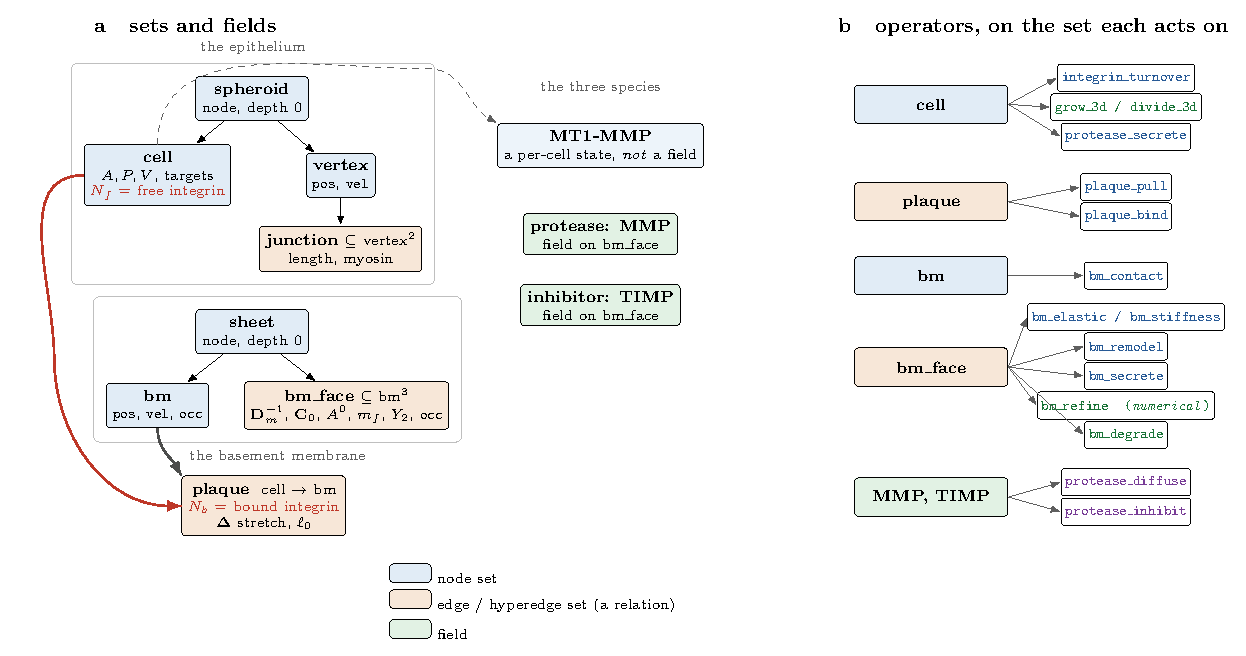
\includegraphics[width=\textwidth]{fig_sets_ops.pdf}
\caption{\textbf{(a)} Every set and field, and which kind each is. A node set carries positions; an
edge or hyperedge set is a \emph{relation} and carries state belonging to neither endpoint --- a
junction to neither cell, a plaque to neither the cell nor the sheet, a triangle to none of its three
nodes. \textbf{(b)} Every operator, on the set it acts on, coloured by kind. Anything carrying a
\emph{force} sits on a set whose elements have positions; anything carrying \emph{mass or number} sits
on the set that owns the quantity. \op{bm\_refine} is the only operator here that is numerical rather
than biological.}
\end{figure}

\subsection*{3.1\; The two diffusible species, and the one that is not}

Proteolysis introduces the first \emph{fields} in this model, and deciding which of the three species
deserves to be one is not a modelling preference --- it is arithmetic.

\smallskip
{\footnotesize
\begin{tabular}{@{}llll@{}}\toprule
species & what it is & where it lives & why\\\midrule
\textbf{MMP} & soluble MMP-2/9, $\sim\!72$ kDa, cuts collagen~IV &
  \textbf{field} on \code{bm\_face} & it diffuses freely, $D\sim10$--$100\,\mu$m$^2$/s\\
\textbf{TIMP} & soluble inhibitor, binds MMP $1{:}1$ &
  \textbf{field} on \code{bm\_face} & likewise --- and it is the \emph{sink}\\
\textbf{MT1-MMP} & membrane-type MMP14, transmembrane &
  a per-\code{cell} \emph{state} & it never enters the extracellular space\\
\bottomrule
\end{tabular}}
\smallskip

\textbf{A soluble protease cannot open a hole, and the arithmetic says so before any run.} In one
$600$~s frame a soluble MMP travels $\sqrt{4Dt}=155$--$490\,\mu$m, against a spheroid $318\,\mu$m
across and a cell of $10\,\mu$m. It is therefore \emph{uniform over the entire sheet within a single
frame}, and a uniform protease dissolves rather than perforates --- the same failure uniform
starvation produced, for the same reason. Localising to one cell would need
$D<0.042\,\mu$m$^2$/s, $240$--$2400\times$ slower than any protein of that size. That is not a
parameter range, it is a different molecule, and the different molecule is MT1-MMP: \emph{tethered},
acting where its cell put it. This is why focal basement-membrane breach is done by membrane-type MMPs
and invadopodia rather than by soluble enzyme.

\textbf{What makes the soluble field worth solving at all is the sink.} With
$\mathrm Dc/\mathrm Dt = D\nabla_s^2c + s - k\,c$ the source decays over $\sqrt{D/k}$, so the field
acquires a \emph{length} instead of filling the sphere --- and $k$ here is not a fitted decay but the
reaction with TIMP. The breach diameter becomes a \emph{prediction} of the MMP/TIMP balance: a
$10\,\mu$m breach needs an effective $k$ of $0.1$--$0.5\,$s$^{-1}$ (half-life $1.4$--$6.9$~s), a
$50\,\mu$m breach $0.004$--$0.02\,$s$^{-1}$ ($35$--$170$~s). A number to check, not to choose.

\textbf{Three new operators, and one costs what the others do not.} \op{protease\_secrete} (Lateral, on
\code{cell}) is the source; \op{protease\_inhibit} (Exchange) is the $1{:}1$ reaction;
\op{protease\_diffuse} (Exchange) is the only operator in this model carrying a \emph{spatial}
coupling, and so the only one whose stability limit involves the mesh. Explicit diffusion needs
$\Delta t D/h^2<\tfrac12$ --- at these $D$, $1{,}300$--$13{,}400$ substeps per frame, \emph{quadrupling
at every $1\!\to\!4$ refinement}, unlike the sheet's own bound which is a rate and mesh-independent. It
is therefore solved semi-implicitly, $(\mathbf I+\Delta t D\mathbf L)c=c_{\rm old}$ by conjugate
gradient on a finite-volume face Laplacian: unconditionally stable, one solve per frame, indifferent
to $h$.

\textbf{The same argument applied to the integrin gives the opposite answer for the opposite reason.}
A receptor is well mixed because it is \emph{confined} to one cell's basal face ($\sqrt{4Dt}=15.5\,\mu$m
over a $10\,\mu$m cell) and needs no field; a soluble protease would be well mixed because it
\emph{travels far}. \textbf{Confinement, not diffusivity, decides whether a species is worth resolving
as a field.}



\subsection*{Proteolysis, and the mechanism the literature forced}

\op{05g\_degrade} put the three species on the entities the confinement argument assigns them and
measured which one can make a hole. The answer was unambiguous and one-sided:

\smallskip
{\footnotesize
\begin{tabular}{@{}lcccc@{}}\toprule
arm & faces dead & under MT1 & elsewhere & sheet breached\\\midrule
both arms      & $317$  & $317$ & $0$    & $6.2\%$\\
soluble only   & $\mathbf 0$ & $0$ & $0$ & $0\%$\\
tethered only  & $317$  & $317$ & $0$    & $6.2\%$\\
no protease    & $0$    & $0$   & $0$    & $0\%$\\
\textbf{no inhibitor} & $\mathbf{5120}$ & $317$ & $\mathbf{4803}$ & $\mathbf{100\%}$\\
\bottomrule\end{tabular}}
\smallskip

The last row is the argument of \S3.1 as an experiment: \textbf{remove TIMP and the sheet dissolves
entirely}, with $4803$ of the deaths nowhere near a cell that expresses MT1-MMP. With the inhibitor
present the diffusible arm kills nothing at all and the tethered arm kills exactly its own footprint.
A soluble protease has no length scale unless something quenches it.

\textbf{Two defects that the runs found rather than the design.} First, neither field had a
\emph{clearance} term, so TIMP accumulated without bound ($0.0318$ at frame $20$, $0.0438$ at frame
$25$) --- its only sink was a $1{:}1$ reaction with an MMP twenty times scarcer, so there was no steady
state for the pair to reach. A first-order clearance is not a refinement: the $\sqrt{D/k}$ that
justifies solving the field \emph{is} that $k$. With it, both fields plateau and drift by
$<10^{-4}$ over twenty frames. Second, a five-point sweep of the MMP:TIMP source ratio over a
hundredfold range returned \emph{identically} $317$ dead at every point, because the direct tethered
cut had been set $350\times$ larger than anything the soluble arm could contribute --- the sweep axis
had no effect on the answer, and the holes were the source stencil in every case.

\subsection*{TIMP-2 is the adaptor as well as the inhibitor, and that predicts a bell}

The pure-inhibitor law of \op{05g} is half of the mechanism. In the canonical model
\cite{karagiannis2004} TIMP-2 is the \emph{bridging adaptor} that makes activation possible: its
C-terminus tethers proMMP-2 and its N-terminus binds MT1-MMP, and the prodomain is then cleaved by a
\emph{second, TIMP-2-free} MT1-MMP \cite{sato2010}. TIMP-2 therefore both presents the zymogen and
poisons the enzyme that must cut it, and the dose response is biphasic. The dissection is clean: an
artificial receptor that tethers proMMP-2 \emph{without} inhibiting MT1-MMP has no descending limb
\cite{cancerres2008}, so the fall-off is inhibition and not saturation.

With $T$ the tethered enzyme and $K$ the MT1--TIMP dissociation constant, occupancy is Langmuir and the
rate needs one occupied site and one free one:
%
\begin{equation}
[\mathrm{MT1\!\cdot\!TIMP}]=T\frac{c_T/K}{1+c_T/K},\quad
[\mathrm{MT1_{free}}]=\frac{T}{1+c_T/K},\quad
\text{act}\;\propto\;T^2c_{\rm pro}\,\frac{c_T/K}{\bigl(1+c_T/K\bigr)^2},
\label{eq:bell}
\end{equation}
%
which is bell-shaped and \textbf{peaks at $c_T=K$}. Both the shape and the location are therefore
predictions, and \op{05g}'s pure-inhibitor law cannot produce a peak at all --- it can only decay ---
so one sweep distinguishes them and \op{05g} is the control.

\textbf{Measured} (\op{05h\_ternary}, eight TIMP levels, four species): the activation rate rises and
falls, $4.5\times10^{-2}\to6.2\times10^{-2}\to2.4\times10^{-2}\to7.5\times10^{-3}\to2.5\times10^{-3}$,
and the pure-inhibitor control over the same sweep is monotone decreasing, as Eq.~\eqref{eq:bell}
requires of it. Two arrangements had to be corrected before the curve could be read at all, and both
are worth recording because they are measurement errors rather than modelling ones: the activation had
to be made \emph{rate-limiting} (at a large $k_{\rm act}$ the whole zymogen pool converts every frame
whatever TIMP does, and saturation erases the dose response); and the rate has to be read \emph{while
the substrate still exists}, since at the TIMP levels where the mechanism works best it destroys every
MT1-bearing face and a late-window average then reports exactly zero at the peak.

\section*{4.\; Gates}


A gate is a number with a threshold decided \emph{before} the run and a stated consequence if it fails.
G1--G4 and G14--G16 run before any physics, as \code{bm\_ops.selftest()}; a rig refuses to start if they
fail.

\smallskip
{\footnotesize
\begin{tabularx}{\textwidth}{@{}llLl@{}}\toprule
& \textbf{gate} & \textbf{threshold} & \textbf{measured}\\\midrule
\multicolumn{4}{@{}l}{\textit{the strain measure} (\S2)}\\
G1 & rigid motion leaves $\lambda=1$ & $<10^{-6}$ & \PASS{$7.5\times10^{-9}$}\\
G2 & dilation by $s$: $\lambda_1=\lambda_2=s$, every face & $<10^{-6}$ &
     \PASS{$2.5\times10^{-8}$} ($J$: $1.1\times10^{-13}$)\\
G3 & affine map gives the singular values of $\mathbf A$ & $<10^{-10}$ & \PASS{$8.9\times10^{-15}$}\\
G4 & force $=-\partial W/\partial\mathbf x$, vs finite difference & $<10^{-6}$ rel. &
     \PASS{$5\times10^{-10}$}\\\midrule
\multicolumn{4}{@{}l}{\textit{the sheet under load} (\op{05a\_sheet})}\\
G5 & stretch fidelity vs the applied $R(t)/R(0)$ & $>0.95$ &
     \PASS{$0.9935$} (MPM: $0.13$, $0.98$)\\
G6 & control $\kappa=0$: nothing pulls, nothing stretches & $=1.00000$ & \PASS{$1.00000$}\\
G7 & control, rigid drive: motion is not deformation & $=1.00000$ & \PASS{$1.00000$}\\
G8 & divergence at $\Delta t M\lambda_{\max}=2$ & stable $<2$, NaN $>2$ &
     \PASS{ran at $1.9$, NaN at $2.1$}\\\midrule
\multicolumn{4}{@{}l}{\textit{the plaque} (\op{05b\_plaque})}\\
G9 & momentum, bookkeeping: $|\sum\mathbf f_{\rm bm}{+}\sum\mathbf f_{\rm epi}|/\sum|\mathbf f|$ &
     $<10\,\varepsilon_{64}$ & \PASS{$1.4\times10^{-16}$}\\
G10& momentum, motion: free pair, centroid drift & $<10^{-12}$ & \PASS{$4.4\times10^{-15}$}\\
G11& control, no plaques: the sheet is not carried & $\lambda\approx1$ &
     $1.25$ vs $3.30$ (marginal)\\
G12& standoff equals $\ell_0$ & $\ell/\ell_0\in[0.9,1.1]$ & \FAIL{$3.43$} --- superseded by
     \S2.3: $96\%$ of nodes were unanchored\\
G13& slip: $\xi=0$ and $\xi>0$ must differ & any separation & \FAIL{none} --- a fixed anchor is a
     pin; slip IS bond turnover\\\midrule
\multicolumn{4}{@{}l}{\textit{the reservoir} (\S2.4, \op{05c\_remesh}, archived \op{05e})}\\
G14& refining an UNLOADED sheet changes $\lambda$ & $<10^{-6}$ ($\sqrt\varepsilon$) &
     \PASS{$6.2\times10^{-9}$}\\
G15& refining a LOADED sheet: $\lambda$ / area / energy & $10^{-12}$, $10^{-9}$, $10^{-6}$ &
     \PASS{$2.3\times10^{-14}$, $0$, $0$}\\
G16& no hanging nodes & exact & \PASS{$0$ bad, $0$ rim}\\
G17& mean edge stays in a band as $R$ triples & $[0.8,1.7]\times$ seeded &
     \PASS{$0.84$} (fixed mesh: $3.33$)\\
G18& refinement does not degrade fidelity & $\ge$ the fixed mesh's &
     \PASS{$0.9985$ vs $0.9873$}\\
G18b& mass $\sum_f m_f$ invariant across a split & exact & \PASS{$0$, bit-identical}\\
G18c& plaque areal density held at $\Sigma^{-2}$ & within $10\%$ &
     \PASS{$0.996$} vs control $0.145$\\
G18d& a split does not move the surface: volume, area, centroid & $<10^{-12}$ rel. &
     \PASS{$2.6\times10^{-16}$, $0$, $9\times10^{-17}$}\\
G18e& $\rho=m/A$ equals $1/J$ & --- & an identity, not a test\\
G28& the sheet stays OUTSIDE the epithelium (signed) & radial gap $>0$ &
     \PASS{$+4.3\times10^{-4}$} (was $-3.6\times10^{-3}$)\\
G29& no plaque ends up on the wrong side & $0\%$ & \PASS{$0.0\%$} (was $89.6\%$)\\
\midrule
\multicolumn{4}{@{}l}{\textit{tearing} (\op{05d\_tear}) --- G19 is the test the MPM sheet never faced}\\
G19& \textbf{same tear, same $\lambda$, under refinement} & onset $\lambda$ within $5\%$ &
     \PASS{$0.52\%$} ($2.110$ vs $2.099$)\\
G20& onset scales with the CRITERION, not element size & monotone / flat &
     \PASS{frame $167$/$227$/$285$ at $1.8$/$2.2$/$2.6$}\\
G21& a hole stays open; the remesher does not heal it & exact &
     \PASS{structural} (rim persists to the last frame)\\
G22& control: criterion above the load kills nothing & exact & \PASS{$0$ of $81{,}920$}\\
G23& the mesh is conforming with a hole in it & $0$ edges with $3$ faces & \PASS{$0$}\\\midrule
\multicolumn{4}{@{}l}{\textit{supply} (\S4, \op{05f\_secrete})}\\
G24& $\rho$ held flat while $A$ triples & within $10\%$ &
     \PASS{$1.0046$} at area $\times11.2$ (starved $0.351$)\\
G25& polarised deposition follows the plaques, uniform does not & $r$ separates &
     \PASS{$+0.880$ vs $-0.053$}\\
G26& starved tears, fed does not, at the same $\lambda$ & --- &
     \PASS{$0$ vs $2515$ faces}\\
G27& dilution and turnover are comparable & ratio within $[0.3,3]$ &
     \FAIL{$0.238$} at $\tau_{\rm bm}\!=\!40$; $0.555$ at $93$\\\midrule
\multicolumn{4}{@{}l}{\textit{adhesion as a density} (\S2.3, \op{05d}, to build)}\\
G28& the sheet stays OUTSIDE the epithelium (signed) & radial gap $>0$ &
     \PASS{$+2.7\times10^{-4}$}\\
G29& no plaque on the wrong side & $0\%$ & \PASS{$0.0\%$}\\
G30& receptor conserved: $N_f+\sum N_b$ moves only by $s_i$, $1/\tau_i$ & exact &
     \PEND{05d}\\
G31& bound fraction depends on LOAD, not on the frame & monotone in stress, plateaus &
     \PEND{05d}\\
G32& slip rate monotone in $k_{\rm off}$, zero at $k_{\rm off}=0$ & separation &
     \PEND{05d}\\
G33& the discrete-plaque model converges to the density model at high $\Sigma^{-2}$ & within $5\%$ &
     \PEND{05d}\\
\bottomrule
\end{tabularx}}
\smallskip

Two conventions make these mean what they say. \textbf{The momentum residual is taken on the adhesion's
own force pair}, inside the substep, before the drive is added --- with the drive's force in the sum it
stops being a statement about the reaction. And \textbf{a rupture threshold is taken from the load
distribution the nominal run measured}, never from a round number: run 127's \code{detach: 0.02} sat
above the largest load in its entire run ($0.017$), so a correctly wired mechanism was reported as a
null.


\begin{figure}[H]\centering

\includegraphics[width=\textwidth]{../log/okuda_ECM/05a_sheet/metrics.png}
\caption{\op{05a\_sheet}, the sheet alone on the recorded epithelial surface. \textbf{a} \PASS{G5}: the
measured $\lambda^{\rm geo}$ lies on the applied $R(t)/R(0)$ to $0.9935$, against $0.13$ for the MPM
sheet moved by an engine delta; the two flat lines at $1.0000$ are \PASS{G6} ($\kappa=0$) and
\PASS{G7} (a rigid drive), i.e. the measure invents no strain and does not mistake motion for
deformation. \textbf{b--c} remodelling: at $\tau_r=25$ frames the standoff improves $1026\times$ while
$\lambda^{\rm geo}$ is unmoved --- the sheet still goes where the tissue puts it and stops fighting.
\textbf{f} \PASS{G8}: divergence at the predicted group $\Delta t M\lambda_{\max}=2$, measured, not
assumed. \textbf{g} the tangent stiffens $19\times$ over the run, which is why the bound has to be
re-measured. \textbf{h} the stiffening law as a ratio, since MPa is not a quantity this box has.}
\end{figure}

\begin{figure}[H]\centering

\includegraphics[width=\textwidth]{../log/okuda_ECM/05b_plaque/metrics.png}
\caption{\op{05b\_plaque}, the adhesion as an edge set. \textbf{1} \PASS{G9}: the residual on the
adhesion's own force pair sits at $1.4\times10^{-16}$, i.e. at double-precision $\varepsilon$ ---
one operator, a delta to both endpoints, and the reaction cannot be half-implemented. \textbf{2}
\PASS{G10}: the same claim as motion, with two free bodies whose mobility-weighted centroid drifts by
$4.4\times10^{-15}$ of the system's own size. \textbf{3} \FAIL{G12}: the standoff is $3.43\,\ell_0$
and not $\ell_0$. \textbf{4} \FAIL{G13}: $\xi=0$ and $\xi>0$ do not separate, because a fixed
barycentric anchor is a tangential pin. \textbf{5} rupture is a clock rather than a load, for want of
turnover. \S4.2 is what each of those three costs, and \S2.3 is the scheme that replaces them.}
\end{figure}

\begin{figure}[H]\centering
\includegraphics[width=\textwidth]{../log/okuda_ECM/_archive_05def/05e_conserve/remesh_model.png}
\caption{\op{bm\_refine} and what it must carry (\op{05e\_conserve}). Red dash-dot lines are the two
refinements, at frames $131$ and $353$. \textbf{Top left} \PASS{G18b}, \PASS{G18d}: $\sum_f m_f$ is
flat through both splits and through an area that grows $\times11$ --- bit-identical --- while the
volume and area grow because the tissue did. \textbf{Top right} \PASS{G18c}: the plaque areal density
is held at $0.996$ of $\Sigma^{-2}$; the fixed-fraction rule 05b used ends at $0.145$. \textbf{Bottom
left} G18e: with nothing secreting, $m/A$ IS $1/J$ identically --- an identity, drawn because it is
the baseline \op{bm\_secrete} has to hold flat. \textbf{Bottom right} the split is invisible in
$\lambda$ (no step at the red lines) while the mean edge length is halved at each.}
\end{figure}

\begin{figure}[H]\centering
\includegraphics[width=\textwidth]{../log/okuda_ECM/_archive_05def/05f_secrete/secrete_model.png}
\caption{\op{bm\_secrete} (\op{05f\_secrete}), in the register of \S3's operator table: the operator
names itself, states the equations it is, and every panel is a measurement that could have come back
wrong. \textbf{Top left} \PASS{G24}: \op{fed} holds $\rho$ at $1.005$ while the area triples, against
$0.351$ starved. \textbf{Top right} \FAIL{G27}: the two removal terms are \emph{not} the same size ---
dilution is $0.238$ of turnover at $\tau_{\rm bm}=40$ frames. \textbf{Bottom left} \PASS{G26}, plotted
against $\lambda$ and not against the frame, because ``starved tears and fed does not'' is a statement
about supply only if the two are compared at the same deformation. \textbf{Bottom right} \PASS{G25}:
polarised deposition ends at $r=+0.88$ with the plaques against uniform's $-0.05$, with the stretch
correlation drawn beside it as the control that separates deposition from mechanics.}
\end{figure}

\begin{figure}[H]\centering

\includegraphics[width=\textwidth]{../log/okuda_ECM/_archive_05def/05d_tear/metrics.png}
\caption{\op{05d\_tear}: tearing, and the gate the MPM sheet was never given. \textbf{Bottom middle}
\PASS{G19}: the same criterion at $5{,}115$ and $20{,}471$ faces tears at $\lambda^{\rm el}=2.110$ and
$2.099$ --- $0.52\%$ apart, against a $5\%$ threshold --- so the tear is set by the material and not by
the discretisation. \textbf{Bottom left} \PASS{G20}, \PASS{G22}: onset moves with the criterion
(frames $167$ / $227$ / $285$ at thresholds $1.8$ / $2.2$ / $2.6$) and a criterion above the largest
stretch reached kills $0$ of $81{,}920$ faces --- which is the run-127 control, run on purpose.
\textbf{Top row} \PASS{G17}, \PASS{G18}: the reservoir holds the edge length at $0.84$ of seeded where
a fixed mesh reaches $3.33$, and refinement improves the fidelity rather than merely preserving it.}
\end{figure}

\subsection*{4.1\; The sweeps behind the table}


\textbf{\op{05a\_sheet}} --- the sheet alone, tethered to the recorded epithelial surface
(\code{smap}: $32\times64$ directions $\times$ $402$ frames, $R$ going $0.0398\to0.1351$ box units, a
ratio of $3.387$), $2562$ nodes, $5120$ faces, no matrix and no plaque.

\smallskip
{\small\begin{tabular}{@{}lccccl@{}}\toprule
run & $\tau_r$ & $\lambda^{\rm geo}$ & $\lambda^{\rm el}$ & standoff & what it says\\\midrule
nominal            & $\infty$ & $3.344$ & $3.344$ & $-1.52\times10^{-3}$ & the sheet stores all of it\\
\op{tau100}        & $100$ fr & $3.384$ & $1.226$ & $-9.96\times10^{-6}$ & $153\times$ better\\
\op{tau25}         & $25$ fr  & $3.384$ & $1.050$ & $-1.48\times10^{-6}$ & $\mathbf{1026\times}$ better\\
\op{beta5}         & $\infty$ & $3.063$ & $3.063$ & $-1.29\times10^{-2}$ & stiffening makes it worse\\
control $\kappa=0$ & --- & $1.0000$ & $1.0000$ & --- & the measure invents nothing\\
control rigid      & --- & $1.0000$ & $1.0000$ & --- & motion is not deformation\\
\bottomrule\end{tabular}}
\smallskip

The third row is a mechanism, not a tuning. Without remodelling the sheet's own hoop stress pulls it
inward faster than a stable tether can hold it out --- which is what \code{HANDOVER.md} concluded from
runs 149--155 and could not test, because \code{membrane\_tau} was $0$ in every one of them. Turning it
on moves the standoff by three orders of magnitude \emph{while $\lambda^{\rm geo}$ stays at $3.38$}: the
sheet still goes where the tissue puts it, it simply stops fighting. $\beta=5$ is the same statement
from the other side --- a sheet that stiffens as it stretches fights harder, and its standoff is
$8.5\times$ worse at $E(\lambda)/E_0=11.3$.

\textbf{\op{05b\_plaque}} --- $2562$ membrane nodes against a $642$-vertex epithelium, $2562$ plaques,
$\ell_0=0.3T$. G9 and G10 pass at machine precision, which is what this run exists for: the reaction is
present, and present as motion and not only as bookkeeping. The density sweep, against the archived
one-sided tether:

\smallskip
{\small\begin{tabular}{@{}lccc@{}}\toprule
anchored & spacing & standoff, two-sided plaque & standoff, one-sided tether (archived)\\\midrule
$100\%$ & $1.5\,T$ & $+1.46\times10^{-3}$ & $-8.2\times10^{-3}$\\
$20\%$  & $3.4\,T$ & $+6.19\times10^{-3}$ & $-4.5\times10^{-2}$\\
$4.6\%$ & $7\,T$ (the measured $\Sigma$) & $+1.68\times10^{-2}$ & $-1.19\times10^{-1}$\\
\bottomrule\end{tabular}}
\smallskip

At this model's plaque density --- which is NOT the density the literature measures, see \S2 ---
which on this mesh is $4.6\%$ of the nodes --- the two-sided plaque sits $7\times$ closer to the surface
than the one-sided tether did. The sign has flipped, and that is \S4.2.

\textbf{\op{05c\_remesh}} --- the same sheet with two levels of reserve ($81{,}920$ face slots,
$40{,}962$ node slots), against the identical run with the reserve switched off. Refinement fires twice,
at frames $110$ and $338$, each time when the mean edge reaches $1.45\times$ its seeded value:
$5120\to20480\to81920$ faces, $2562\to10242\to40962$ nodes.

\smallskip
{\small\begin{tabular}{@{}lccccc@{}}\toprule
& faces & mean edge / seeded & $\lambda^{\rm geo}$ & fidelity vs applied $3.387$ & standoff\\\midrule
reservoir, 2 levels & $81{,}920$ & $\mathbf{0.84}$ & $3.3817$ & $\mathbf{0.9985}$ &
  $-9.89\times10^{-5}$\\
fixed mesh (05a)    & $5120$     & $3.33$          & $3.3440$ & $0.9873$ & $-1.52\times10^{-3}$\\
\bottomrule\end{tabular}}
\smallskip

G17 passes. G18 was written as ``the refined run must match the fixed-mesh run to $1\%$'' and the two
are $1.12\%$ apart --- \textbf{which is the gate being wrong, not the run.} The fixed mesh is not the
truth: a coarse triangle chords a curved, stretching surface and under-reports how much it stretched, so
refinement moves the fidelity from $0.9873$ to $0.9985$ and the residual error from $1.3\%$ to $0.15\%$.
The gate is therefore restated against the \emph{applied} stretch, where refinement can only help, and
G18 as originally phrased would have rejected an improvement. The standoff improves by $15\times$ in the
same run, for the same reason: more nodes tethered to the surface track it more closely.

\textbf{\op{05e\_conserve}} --- the reservoir and the plaque in one rig, so that a refinement has
something to break, with mass as the state (Eq.~\ref{eq:massstate}) and \op{plaque\_seed} holding
$\Sigma^{-2}$. Over $401$ frames it refines twice, at frames $131$ and $353$, and the sheet's area goes
$\times11$:

\smallskip
{\small\begin{tabular}{@{}llll@{}}\toprule
& threshold & measured & \\\midrule
G18b & $\sum_f m_f$ across a split & exact & $\mathbf{0}$, and $\mathbf{0}$ over the whole run\\
G18c & plaque density $\times\Sigma^{2}$ & within $10\%$ & $\mathbf{0.996}$ \ ($104\to1056$ plaques)\\
G18c & \emph{control}: 05b's fixed-fraction rule & --- & $0.145$\\
G18d & volume / area / centroid across a split & $<10^{-12}$ &
  $2.6\times10^{-16}$, $\mathbf 0$, $9.1\times10^{-17}$\\
G18e & $\rho=m/A$ against $1/J$ & --- & $1.4\times10^{-16}$: an identity, not a test\\
\bottomrule\end{tabular}}
\smallskip

Two things in that table are worth saying in words. \textbf{Mass is bit-identical across a split and
across the whole run}, which is what licenses \op{bm\_secrete} to be built on top: a substrate that lost
material when it refined could not tell secretion from arithmetic. And \textbf{the control is a larger
failure than predicted}: 05b's rule loses a factor of $6.9$, not the factor of $4$ per refinement one
would guess, because a fixed fraction is wrong at each split \emph{and} continuously as the area grows
between them.

\textbf{One operator changed kind because of this.} \op{bm\_secrete} was written as a \emph{Divide} ---
wake reserve faces to add material, which is what a particle model must do. With mass carried as a
scalar on a face it is a \emph{Lateral} operator: it raises $m_f$ on faces that already exist, and the
reservoir is needed for resolution and not for supply. That is a simplification the $\rho$-as-state form
would have hidden.

\subsection*{4.2\; Three gates that failed, and none of them is a parameter}


\textbf{The standoff is $3.43\,\ell_0$, not $\ell_0$ (G12).} The sheet lags the expanding epithelium, so
every plaque is \emph{extended} rather than sitting at its rest length, and the extension is what
carries the sheet outward. $\ell_0$ therefore sets the standoff only in a quasi-static sheet; in a
growing one it is $\ell_0$ plus a lag, and the lag is the same hoop stress \S4.1 isolates. The prediction
is sharp and is the next run: \op{05b} with $\tau_r=25$ should collapse $3.43\to\sim\!1$.

\textbf{Friction is currently unmeasurable in this rig (G13).} With $\xi=0$ the sheet twisted
$28.49^\circ$ against a drive of $28.50^\circ$ --- it followed the epithelium essentially exactly with
no friction at all. The reason is structural: a plaque anchored to a \emph{fixed} barycentric point is a
pin in the tangential direction, because that anchor is a material coordinate that rotates with the
face. $\xi$ can only set how fast the sheet equilibrates to a pin, never whether it slides.
\textbf{Slip requires the anchor to move over the epithelial surface}, i.e. \op{plaque\_seed} as
turnover. \S5 of \code{note\_spheroid\_bm\_ecm} asked for friction where what was needed was turnover;
that is a correction to the design, and the run is what found it.

\textbf{Turnover does not merely match growth --- it dominates it, and \S9 of
\code{note\_spheroid\_bm\_ecm} says otherwise.} That note argues the two removal terms of the mass
balance are the same size, ``turnover is not a correction to growth; it is the same size as growth,
which is why the sheet can accommodate it at all''. Measured on the geometry rather than estimated:
$\dot A/A$ has median $5.96\times10^{-3}$ per frame against $1/\tau_{\rm bm}=2.5\times10^{-2}$, a ratio
of $\mathbf{0.238}$ --- turnover runs $4.2\times$ faster than dilution at the mid-range half-life, and
$1.8\times$ faster ($0.555$) at $\tau_{\rm bm}=93$ frames, the $10$~h end. The claim therefore holds
only near the slow end of the literature's $3$--$10$~h range, and the correct statement is that
\emph{turnover dominates growth by a factor of two to four}. It is the same conclusion for the sheet ---
a membrane that replaces itself faster than it is diluted can hold its density --- reached by a
different margin than the note asserts.

\textbf{Rupture is all-or-nothing for a structural reason.} At a threshold of $0.0052$, inside the
measured load range (the nominal's p99 reaches $0.0120$), \emph{every} plaque broke. With a load that
rises monotonically as the tissue grows and nothing that re-forms a bond, any threshold inside the range
is reached by every plaque eventually: the fraction bound is a function of time and not of load. A
partial-rupture regime needs a distribution of thresholds across plaques, or turnover. Reporting a
fraction bound without one of those would be reporting a clock.

\subsection*{4.3\; What this licenses, and what it does not}


Licensed: the sheet's deformation is measured rather than advected (G1--G5); its stability limit is a
rate that is measured rather than asserted (G8); its adhesion is a relation that returns its reaction to
machine precision (G9, G10); and its \emph{size} is now a state variable that can be changed without
disturbing the mechanics at all (G14--G16, with area and energy bit-identical across a split). Those are
the four things the archived line could not get, and they are what \op{04} needs before a membrane can
be put into it.

Not licensed: the standoff is not yet $\ell_0$; slip needs turnover, not friction; rupture needs a
threshold distribution; there is no secretion, so Eq.~\eqref{eq:mass} is a baseline ($\rho\to1/11.1$)
and not yet a mechanism; refinement is global rather than adaptive, and a crack tip will want local;
there is no coarsening, so the sheet can only get finer; there is no bending stiffness, so it cannot
fold, and a hole's rim has no line tension; there is no matrix and no \op{fibril}, so nothing yet
removes the epithelium's direct push on the stroma; and the epithelium in \op{05b} is a driven
icosphere, not the vertex model --- \op{mesh\_contact} certifies that interface separately, and joining
the two is what \op{05g} does.

\section*{5.\; References}


{\small
\begin{thebibliography}{99}\setlength{\itemsep}{0pt}
\bibitem{karagiannis2004} Karagiannis, E.D., Popel, A.S. (2004) A theoretical model of type I
collagen proteolysis by matrix metalloproteinase (MMP) 2 and membrane type 1 MMP in the presence of
tissue inhibitor of metalloproteinase 2. \emph{J. Biol. Chem.} \textbf{279}(37):39105--39114. --- the
canonical ODE network for MT1-MMP / TIMP-2 / proMMP-2 / MMP-2, and the source of the reaction topology
used here.
\bibitem{sato2010} Sato, H., Takino, T. (2010) Coordinate action of membrane-type matrix
metalloproteinase-1 (MT1-MMP) and MMP-2 enhances pericellular proteolysis and invasion.
\emph{Cancer Sci.} \textbf{101}(4):843--847.
\bibitem{cancerres2008} Activation of MMP-2 by MT1-MMP through an artificial receptor for proMMP-2
generates active MMP-2. \emph{Cancer Res.} (2008) \textbf{68}(21):9096. --- the dissection showing the
descending limb is MT1-MMP inhibition and not receptor saturation.
\bibitem{stvk} Bonet, J., Wood, R.D. (2008) \emph{Nonlinear Continuum Mechanics for Finite Element
Analysis}, 2nd ed. Cambridge University Press. --- the constant-strain-triangle membrane of \S3.
\bibitem{candiello2007} Candiello, J., Balasubramani, M., Schreiber, E.M., Cole, G.J., Mayer, U.,
Halfter, W., Lin, H. (2007) Biomechanical properties of native basement membranes.
\emph{FEBS J.} \textbf{274}(11):2897--2908.
\bibitem{bell1978} Bell, G.I. (1978) Models for the specific adhesion of cells to cells.
\emph{Science} \textbf{200}(4342):618--627. --- the force-dependent off-rate
$k_{\rm off}=k^0_{\rm off}e^{f/f_b}$ that makes rupture a load and not a clock.

\bibitem{changede2017} Changede, R., Sheetz, M. (2017) Integrin and cadherin clusters: a robust
way to organize adhesions for cell mechanics. \emph{BioEssays} \textbf{39}(1):1600123. --- nascent
adhesions are $\sim\!100$ nm and contain $\sim\!50$ integrins; large adhesions are loose aggregates of
such clusters.
\bibitem{nanoclusters2025} \emph{Differential spatial regulation and activation of integrin
nanoclusters inside focal adhesions.} eLife reviewed preprint 105270. --- STORM: nanocluster median
size $35$--$40$ nm, centre-to-centre $\sim\!555$ nm, spacing set cell-intrinsically. Cited as a
preprint.
\bibitem{kanchanawong2010} Kanchanawong, P., Shtengel, G., Pasapera, A.M., Ramko, E.B., Davidson, M.W.,
Hess, H.F., Waterman, C.M. (2010) Nanoscale architecture of integrin-based cell adhesions.
\emph{Nature} \textbf{468}:580--584. --- iPALM, and it measures the VERTICAL architecture: a
$\sim\!40$ nm integrin-to-actin core, actin peaking at $z=97$ nm. It contains no lateral plaque
diameter and no lateral spacing, so it licenses $\ell_0$ and NOT $\Sigma$.
\bibitem{matsubayashi2020} Matsubayashi, Y., S\'anchez-S\'anchez, B.J., Marcotti, S., Serna-Morales, E.,
Dragu, A., D\'iaz-de-la-Loza, M.-C., Vizcay-Barrena, G., Fleck, R.A., Stramer, B.M. (2020) Rapid
homeostatic turnover of embryonic ECM during tissue morphogenesis. \emph{Dev. Cell} \textbf{54}(1):33--42.
\bibitem{kelley2019} Kelley, L.C., Chi, Q., C\'aceres, R., Hastie, E., Schindler, A.J., Jiang, Y.,
Matus, D.Q., Plastino, J., Sherwood, D.R. (2019) Adaptive F-actin polymerization and localized ATP
production drive basement membrane invasion in the absence of MMPs. \emph{Dev. Cell} \textbf{48}(3):313--328.
\bibitem{yurchenco2011} Yurchenco, P.D. (2011) Basement membranes: cell scaffoldings and signaling
platforms. \emph{Cold Spring Harb. Perspect. Biol.} \textbf{3}(2):a004911.
\bibitem{keene1987} Keene, D.R., Sakai, L.Y., Lunstrum, G.P., Morris, N.P., Burgeson, R.E. (1987)
Type VII collagen forms an extended network of anchoring fibrils. \emph{J. Cell Biol.}
\textbf{104}(3):611--621.
\bibitem{rivara1984} Rivara, M.-C. (1984) Algorithms for refining triangular grids suitable for adaptive
and multigrid techniques. \emph{Int. J. Numer. Methods Eng.} \textbf{20}(4):745--756. --- the local
alternative to the global $1\!\to\!4$ split of \S2.4, for when a crack tip needs it.
\bibitem{okuda2013} Okuda, S., Inoue, Y., Eiraku, M., Sasai, Y., Adachi, T. (2013) Reversible network
reconnection model for simulating large deformation in dynamic tissue morphogenesis.
\emph{Biomech. Model. Mechanobiol.} \textbf{12}(4):627--644.
\bibitem{hgo2000} Holzapfel, G.A., Gasser, T.C., Ogden, R.W. (2000) A new constitutive framework for
arterial wall mechanics and a comparative study of material models. \emph{J. Elasticity} \textbf{61}:1--48.
\end{thebibliography}}


\end{document}
